
\tikzstyle{block} = [draw, fill=blue!20, rectangle, 
    minimum height=2em, minimum width=3em]
\tikzstyle{sum} = [draw, fill=blue!20, circle, node distance=1cm]
\tikzstyle{input} = [coordinate]
\tikzstyle{output} = [coordinate]
\tikzstyle{out} = [coordinate]
\tikzstyle{pinstyle} = [pin edge={to-,thin,black}]

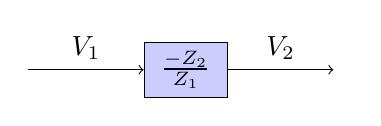
\begin{tikzpicture}[auto, node distance=2cm]
    \node [input, name=input] {};
    \node [block, right of=input] (control) {$\frac{-Z_2}{Z_1}$};
    \node [right of=control] (output) {};
    \draw [draw,->] (input) -- node {$V_1$} (control);
    \draw[draw,->](control) -- node{$V_2$}(output);
\end{tikzpicture}
